\documentclass[12pt]{article}
\usepackage[spanish]{babel}
\usepackage{geometry}
\geometry{a4paper, margin=1in}
\usepackage{graphicx}
\usepackage{xcolor}
\usepackage{titlesec}
\usepackage{parskip}
\usepackage{multicol}
\usepackage{cite}
\usepackage{float}

\definecolor{highlight}{RGB}{255, 255, 0}

\titleformat{\section}{\normalfont\Large\bfseries}{\thesection}{1em}{}
\titleformat{\subsection}{\normalfont\large\bfseries}{\thesubsection}{1em}{}

\begin{document}

% Logos
\begin{minipage}{0.45\textwidth}
    
\includegraphics[width=0.4\textwidth]{inFiles/Figures/epnLogo.jpg}
\end{minipage}
\hfill
\begin{minipage}{0.45\textwidth}
    \raggedleft
    
\includegraphics[width=0.4\textwidth]{inFiles/Figures/FIS_logo.jpg}
\end{minipage}

\vspace{0.5cm}

% Títulos principales
\begin{center}
    \textbf{ESCUELA POLITÉCNICA NACIONAL}\\[0.2cm]
    \textbf{FACULTAD DE INGENIERÍA DE SISTEMAS}\\[0.2cm]
    \textbf{INGENIERÍA {\textbf{EN COMPUTACIÓN}}}
\end{center}

\vspace{0.5cm}
\hrule
\vspace{0.5cm}

% Datos principales
\noindent\textbf{PERÍODO ACADÉMICO:} 2025-A\\[0.2cm]
\noindent\textbf{ASIGNATURA:} Compiladores\\[0.2cm]
\noindent\textbf{TIPO DE INSTRUMENTO:} Tarea 1\\[0.2cm]
\noindent\textbf{FECHA DE ENTREGA LÍMITE:} 12/05/2025\\[0.2cm]
\noindent\textbf{ALUMNO:} Murillo Tobar Juan

\vspace{0.5cm}
\hrule
\vspace{1cm}


% Secciones
\section*{TEMA}
JFLAP
\vspace{0.5cm}


\section*{DESARROLLO}
Construimos los compiladores hechos en clase y sacamos conclusiones.

El primero fue el que reemplazaba los 0 por x y los 1 por y
\begin{figure}[H]
\centering
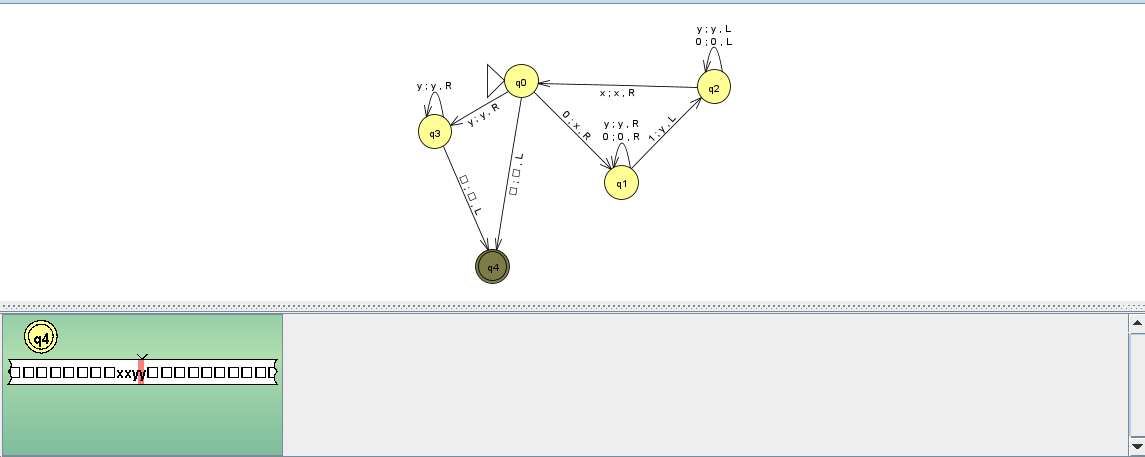
\includegraphics[width=1\textwidth]{./inFiles/Figures/Cap1.png}
\caption{Captura de JFLAP}
\end{figure}

El segundo fue una modificación del anterior para aceptar cadenas $0^n1^n0^n$

\begin{figure}[H]
\centering
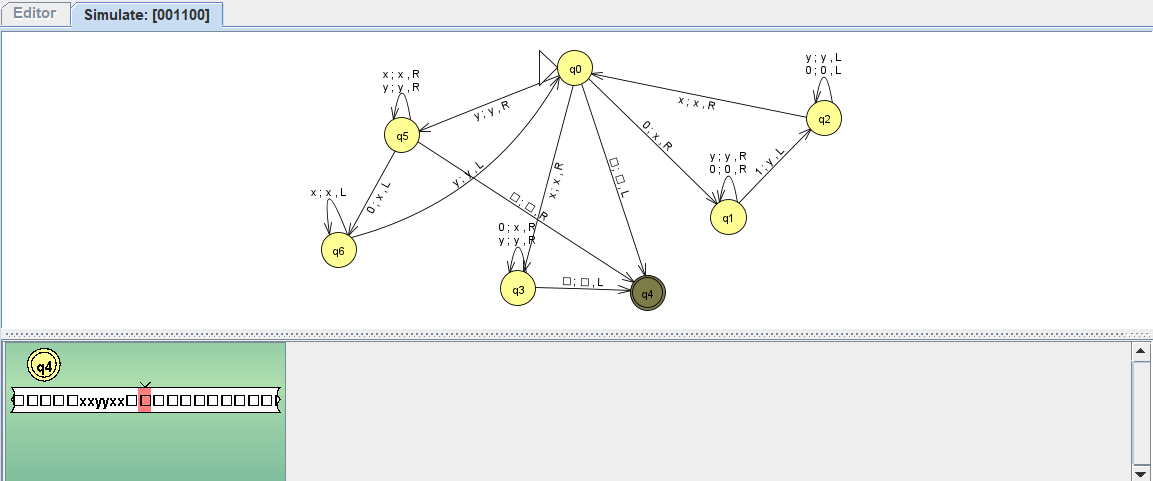
\includegraphics[width=1\textwidth]{./inFiles/Figures/Cap2.png}
\caption{Captura de JFLAP}
\end{figure}

El tercero fue una maquina que se propuso en clase al final para probar las cadenas 01110 y 00110
\begin{figure}[H]
\centering
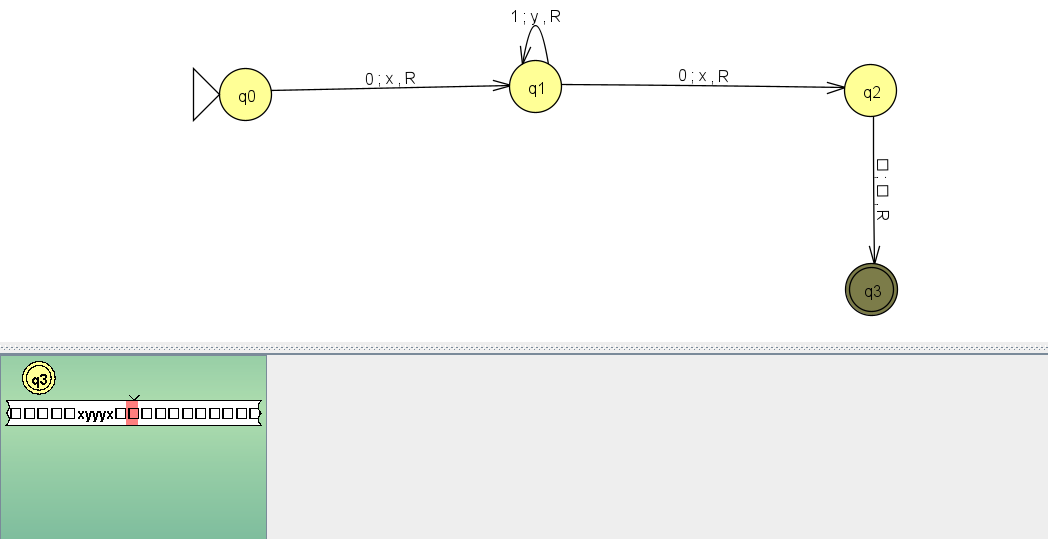
\includegraphics[width=1\textwidth]{./inFiles/Figures/Cap3.png}
\caption{Prueba de la cadena 01110}
\end{figure}

\begin{figure}[H]
\centering
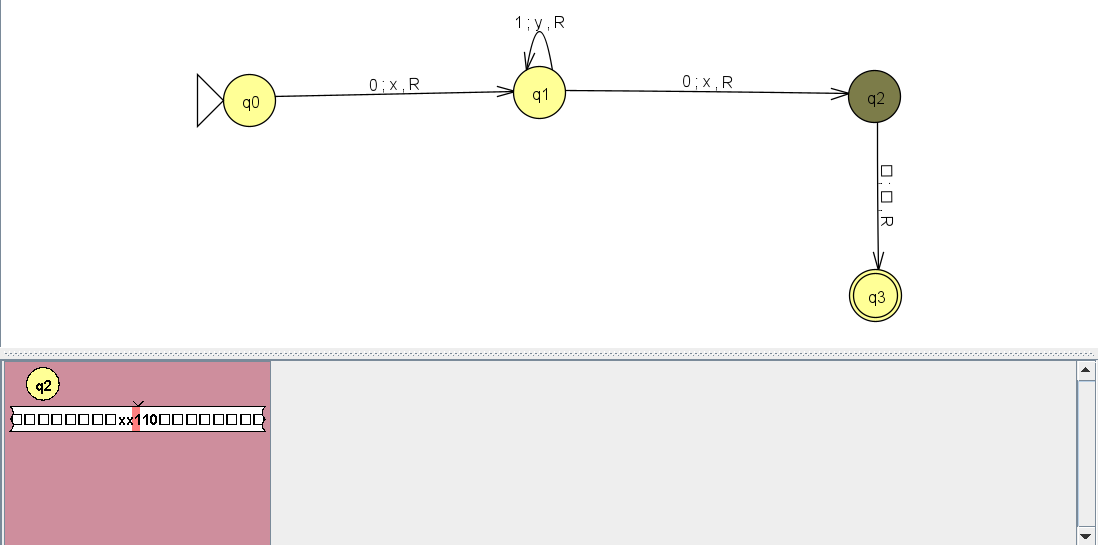
\includegraphics[width=1\textwidth]{./inFiles/Figures/Cap4.png}
\caption{Prueba de la cadena 00110}
\end{figure}

\vspace{0.5cm}


\vspace{0.5cm}


\renewcommand{\refname}{\MakeUppercase{REFERENCIAS}}
%\bibliographystyle{IEEEtran}
%\bibliography{inFiles/References/references.bib}

\end{document}
